\subsection{Results}
Here, the process that a curve undergoes from initialisation to the generation of the final final velocity profile will be demonstrated, drawing upon the theoretical underpinnings of the previous sections.
Firstly, a curve is obtained through plotting or by extraction from image features. The curve that will be taken through the optimisation process can be seen in Figure \ref{fig:example}. The curve has eight control points and has a complex shape that will incur several changes in the limiting axis, demonstrating the ability of our optimisation process to drive the machine to the limits of its physical limitations.

\begin{figure}  
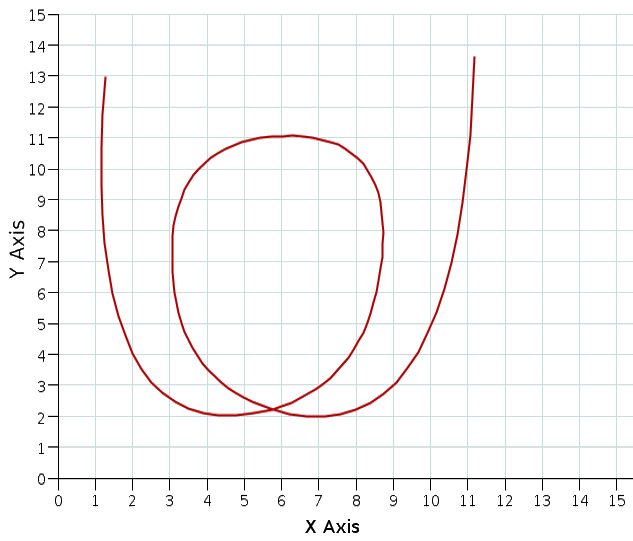
\includegraphics[width=\textwidth]{figures/optimisation/exampleSpline.png}
\caption[Optimisation example curve]{ This spline has 7 control points and 10 knots. This example will be used to demonstrate the properties of URBS curves and the optimisation process.
\label{fig:example}}
\end{figure}

The spline is decomposed into its X and Y axis coordinates, giving the positions that each axis should achieve at each point on the curve. At this level of zoom the error in the final curve that our system produces is nearly imperceptible and is included on the position profiles seen in Fig.\ref{fig:xy_s}. The deviation from the correct path is not an artefact of the optimisation process. The velocity profile sampling which is required to pass the movement information across to the plant discretises the velocity information, which causes accumulating integration error.\footnote{Further work would include an interpolation scheme based on the sampling rate that would adjust these profiles such that the machine would be back on the curve after each sampling period. This implementation is not trivial as the adjustments to the velocity discretisation may cause the acceleration constraints to become exceeded.} However it can be seen in Fig.\ref{fig:xy_s} that the final effect is slight. The effects are also reset at the culmination of each curve. Thus the introduced error was considered to be within allowable bounds for our purposes.

\begin{figure}  
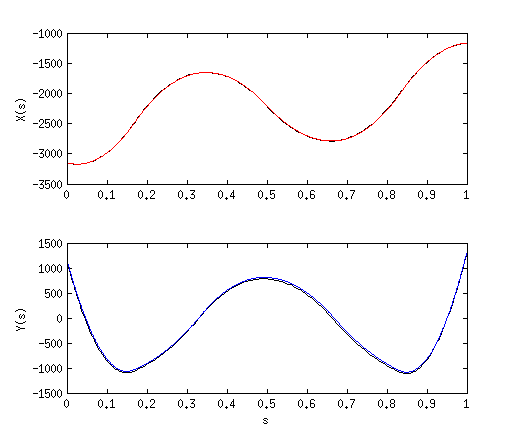
\includegraphics[width=\textwidth]{figures/optimisation/xy_s.png}
\caption[Indexed curve position and theoretical final path]{
The X axis (TOP) and Y axis (BOTTOM) displaying the correct trajectory in colour and the approximated path that will be followed in black, given a velocity profile that is sampled at 25Hz.
\label{fig:xy_s}}
\end{figure} 

Given the path, our algorithm can extract the path velocity and acceleration ($\textbf{q}'(t)$ and $\textbf{q}''(t)$) at each discretisation point for the SeDuMi solver. The curves for the path in the example spline seen in Fig~\ref{fig:example} can be seen in Fig~\ref{fig:xy_dds_ds}. These values are extracted by taking the derivative of the URBS weighting equations with respect to $s$.

\begin{figure}  
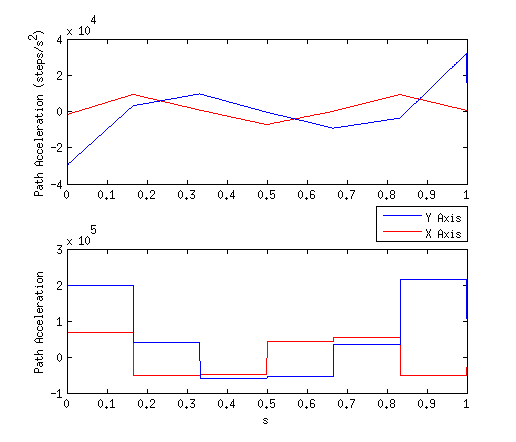
\includegraphics[width=\textwidth]{figures/optimisation/xy_dds_ds.png}
\caption[Indexed curve velocity and acceleration]{
The curve velocity (TOP) and acceleration (BOTTOM) for the example curve. Note the discrete jumps in level for the acceleration and the corresponding changes in gradient for the velocity.
\label{fig:xy_dds_ds}}
\end{figure}

Given this construction of the problem, SeDuMi can solve for the optimal discrete $\dot{s}^*(s)$. The solution given for the example curve can be seen in Fig.~\ref{fig:sdot_st}.
The final calculation to achieve the desired $s^*(t)$ requires that we compute the expected time $t$ for each $s$ via the inverse relation
\begin{align*}
t(s) &= \int_0^s\frac{1}{\dot{s}^*(s)}du\\ 
\end{align*}

\begin{figure}  
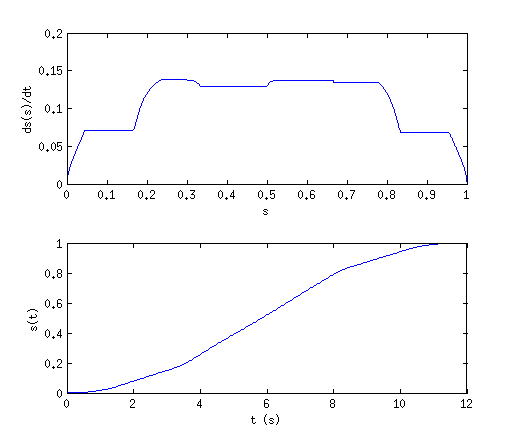
\includegraphics[width=\textwidth]{figures/optimisation/sdot_st.png}
\caption[$\dot{s}^*(s)$ and $s^*(t)$]{
The optimal curve velocity (TOP) and the retrieved path trajectory (BOTTOM) for the example curve.
\label{fig:sdot_st}}
\end{figure}

Since $\dot{s}^*(s)$ is defined in a piecewise non-linear fashion due to its relation to the piecewise linear trajectory $b(s)$, we obtain a mapping between $t$ and $s$ for arbitrary $t$ via the algorithm outlined in Appendix C. The output $s(k\Delta T)$ can be seen in Fig.~\ref{fig:sdot_st}. Though the solution can be solved into a piecewise closed form, an algorithm that solves for a given discrete sampling rate $k\Delta T$ was used instead. This allows us to specify a desired velocity profile sampling frequency and hence use the subsequently calculated values of $s(k\Delta T)$ to generate the sampled velocity profile via 
\begin{align*}
\frac{d\textbf{q}\left(k \Delta T\right)}{dt} &= \frac{\textbf{q}\left(s(k\Delta T)\right)}{ds}\frac{ds(k\Delta T)}{dt}
\end{align*}
Hence, we have generated the optimal axis velocity curves that can be sent to the unit in order to faithfully follow a URBS curve with a time optimal trajectory.
An output of the optimal trajectory $\dot{\textbf{q}}(k\Delta T)$ and $\ddot{\textbf{q}}(k\Delta T)$ can be seen in Fig.~\ref{fig:bangbang}.


\begin{figure}  
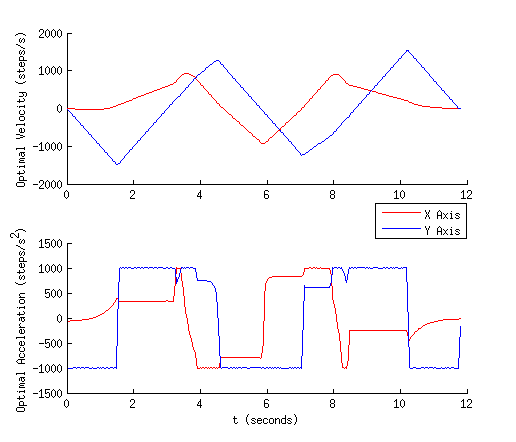
\includegraphics[width=\textwidth]{figures/optimisation/bangbang_xy_ddt_dt.png}
\caption[$\dot{\textbf{q}}^*(t)$ and $\ddot{\textbf{q}}^*(t)$]{
The optimal axis velocity (TOP) and the optimal path acceleration (BOTTOM) for the example curve.
\label{fig:bangbang}}
\end{figure}



